% Koko
\documentclass[ichigo,normal,cn]{elegantnote}
\usepackage{tikz}
\definecolor{light-gray}{gray}{0.95}
\newcommand{\code}[1]{\colorbox{light-gray}{\texttt{#1}}}
\newfontfamily\courier{Courier New}
\lstset{linewidth=1.1\textwidth,
	numbers=left,
	basicstyle=\small\courier,
	numberstyle=\tiny\courier,
	keywordstyle=\color{blue}\courier,
	commentstyle=\it\color[cmyk]{1,0,1,0}\courier, 
	stringstyle=\it\color[RGB]{128,0,0}\courier,
	frame=single,
	backgroundcolor=\color[RGB]{245,245,244},
	breaklines,
	extendedchars=false, 
	xleftmargin=2em,xrightmargin=2em, aboveskip=1em,
	tabsize=4, 
	showspaces=false
	basicstyle=\small\courier
}
\title{程序设计实践课程作业 \\ 
Pastebin.rs 测试文档}
\author{2017211305 班 \\ 2017211240 于海鑫}
\version{$\alpha$}
\begin{document}
\maketitle


\section{测试环境}

操作系统: KUbuntu 19.10

编程语言:Rust

开发环境:VS Code

\section{测试过程}
其实对于 rust 而言,其在设计层面上已经成功地将在别的语言中是运行时错误的问题(例如悬垂指针)转化为了编译时的问题。一旦程序成功编译,很多时候程序就是可以直接运行的,最多可能会出现一些小的逻辑错误。但为了严谨我们还是实现了一部分的测试测试用例。
\subsection{单元测试}
单元测试(Unit Testing)是一种软件测试方法,通过这种测试方法测试各个源代码单元,一个或者多个模块的集合,使用程序来测试程序,来保证它们的可用性。在 Rust 语言内部已经给我们集成了相关的特性来进行单元测试,例如最简单的进行单元测试的代码如下:

\begin{lstlisting}
pub fn add_two(a: i32) -> i32 {
    internal_adder(a, 2)
}

fn internal_adder(a: i32, b: i32) -> i32 {
    a + b
}

#[cfg(test)]
mod tests {
    use super::*;

    #[test]
    fn internal() {
        assert_eq!(4, internal_adder(2, 2));
    }
}
\end{lstlisting}

我们对于主要的函数都实现了单元测试用例。例如测试从数据库获取 \code{User} 结构的代码如下:

\begin{lstlisting}
#[cfg(test)]
mod test {
    use super::*;
    use async_std::task;
    use crate::utils::test_util;

    async fn get_test_user(pool: &ConnPool) -> Result<User, Error> {
        User::get_user("test".to_string(), pool).await
    }

    #[test]
    fn check_user() -> Result<(), Error> {
        let pool = test_util::new_conn_pool();
        let test_user = User {
            username: "test".to_string(),
            password: "password".to_string()
        };
        let user = task::block_on(get_test_user(&pool))?;
        assert_eq!(user.username(), test_user.username());
        assert_eq!(user.password(), test_user.password());
        let _ = task::block_on(user.delete(&pool));
        Ok(())
    }

}
\end{lstlisting}

其示例运行结果如下:

\begin{lstlisting}
name1e5s@sumeru:~/pastebin.rs$ cargo test
    Finished test [unoptimized + debuginfo] target(s) in 0.10s
     Running target/debug/deps/pastebin_server-36632eb4686bcbf5

running 1 test
test models::users::test::check_user ... ok

test result: ok. 1 passed; 0 failed; 0 ignored; 0 measured; 0 filtered out
\end{lstlisting}

我们对我们认为需要进行单元测试的函数都实现了对应的测试机制。

\section{系统测试}

\subsection{API 接口}
我们通过使用 \code{Invoke-WebRequest} 发送样例数据的方式对我们的 API 进行测试,部分测试结果如下:
\begin{lstlisting}
PS C:\Users\name1> Invoke-WebRequest -Uri "http://name1e5s.fun:8888/api/user/name1e5s"


StatusCode        : 200
StatusDescription : OK
Content           : {"author":"name1e5s","list":[{"author_name":"name1e5s","content":"www","created_at"
                    :"2019-12-11T09:42:35","id":"0858f209f59a4d669addb83dea8d724d","lang":"language-mar
                    kup","title":null},{"author_name":...
RawContent        : HTTP/1.1 200 OK
                    transfer-encoding: chunked
                    Content-Type: application/json
                    Date: Wed, 11 Dec 2019 13:09:49 GMT

                    {"author":"name1e5s","list":[{"author_name":"name1e5s","content":"www","created_at"
                    :...
Forms             : {}
Headers           : {[transfer-encoding, chunked], [Content-Type, application/json], [Date, Wed, 11 Dec
                     2019 13:09:49 GMT]}
Images            : {}
InputFields       : {}
Links             : {}
ParsedHtml        : mshtml.HTMLDocumentClass
RawContentLength  : 1469



PS C:\Users\name1> Invoke-WebRequest -Uri "http://name1e5s.fun:8888/api/paste/0858f209f59a4d669addb83dea8d724d"


StatusCode        : 200
StatusDescription : OK
Content           : {"author_name":"name1e5s","content":"www","created_at":"2019-12-11T09:42:35","id":"0858f209f59a4d669addb83dea8d724d","lang":"language-markup","title":null}
RawContent        : HTTP/1.1 200 OK
                    transfer-encoding: chunked
                    Content-Type: application/json
                    Date: Wed, 11 Dec 2019 13:10:28 GMT

                    {"author_name":"name1e5s","content":"www","created_at":"2019-12-11T09:42:35","id":"0...
Forms             : {}
Headers           : {[transfer-encoding, chunked], [Content-Type, application/json], [Date, Wed, 11 Dec 2019 13:10:28 GMT]}
Images            : {}
InputFields       : {}
Links             : {}
ParsedHtml        : mshtml.HTMLDocumentClass
RawContentLength  : 155
\end{lstlisting}

测试结果符合预期。

\subsection{网页端}
我们通过手动登录网页的方式进行测试,可以发现结果与预期相符。

主界面效果如图~\ref{fig:main}~。

\begin{figure}[!htbp]
    \centering
    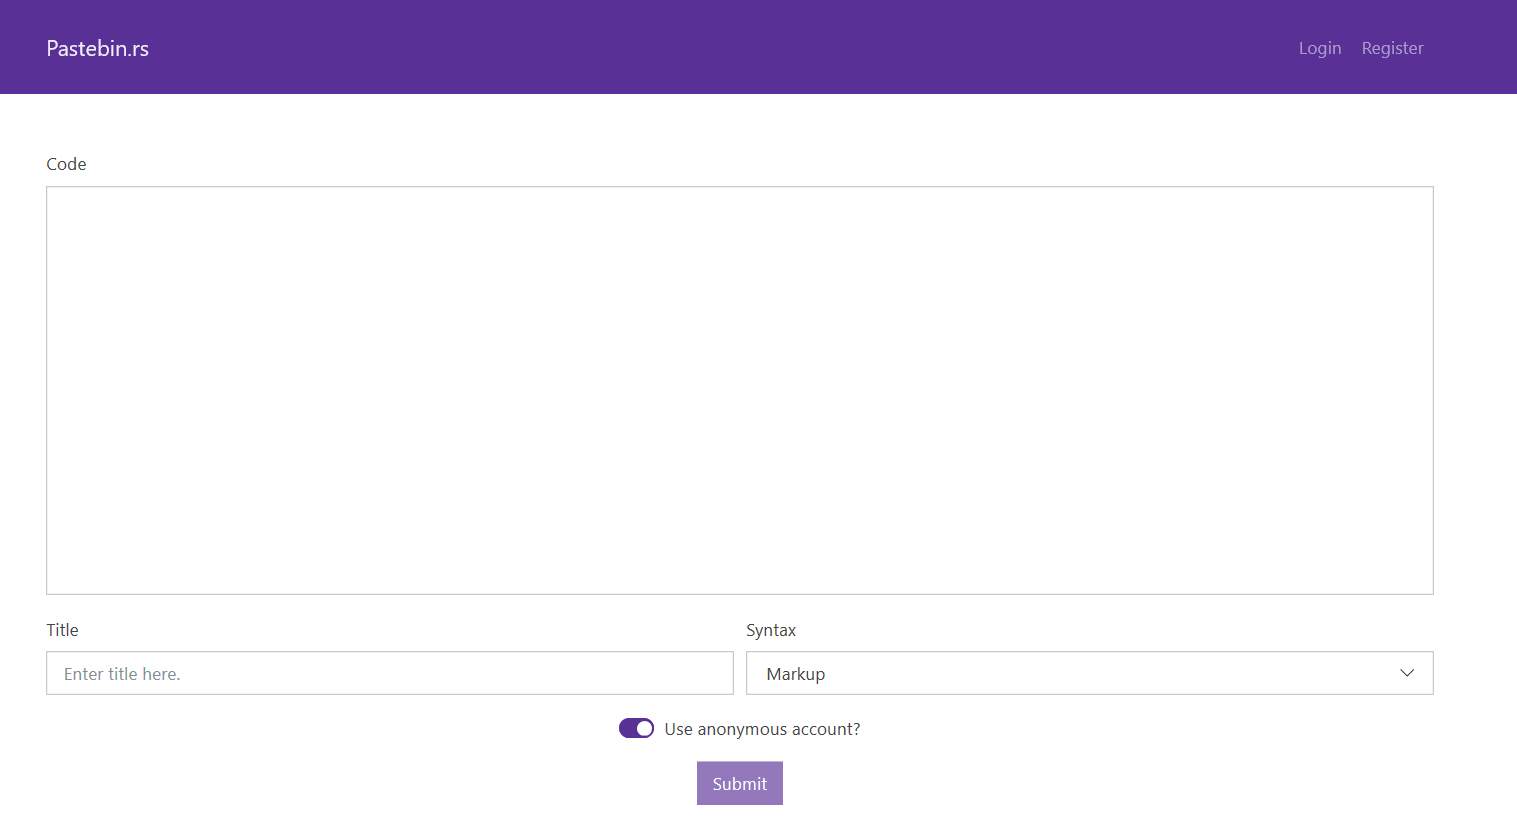
\includegraphics[width=.8\textwidth]{main}
    \caption{主界面}
    \label{fig:main}
\end{figure}

点击左上角登录即可进入登录界面,如图~\ref{fig:login}~。

\begin{figure}[!htbp]
    \centering
    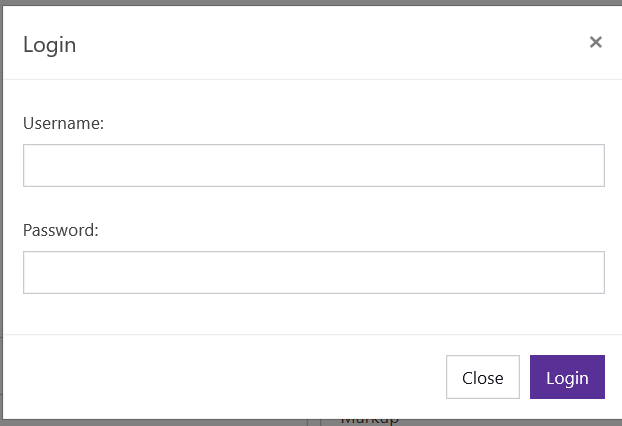
\includegraphics[width=.5\textwidth]{login}
    \caption{登录界面}
    \label{fig:login}
\end{figure}

点击下方的提交按钮即可提交代码,提交后会直接跳转到对应代码的展示界面。点击右上角的用户名,可以进入用户对应的代码片段的展示列表,如图~\ref{fig:user}~。

\begin{figure}[!htbp]
    \centering
    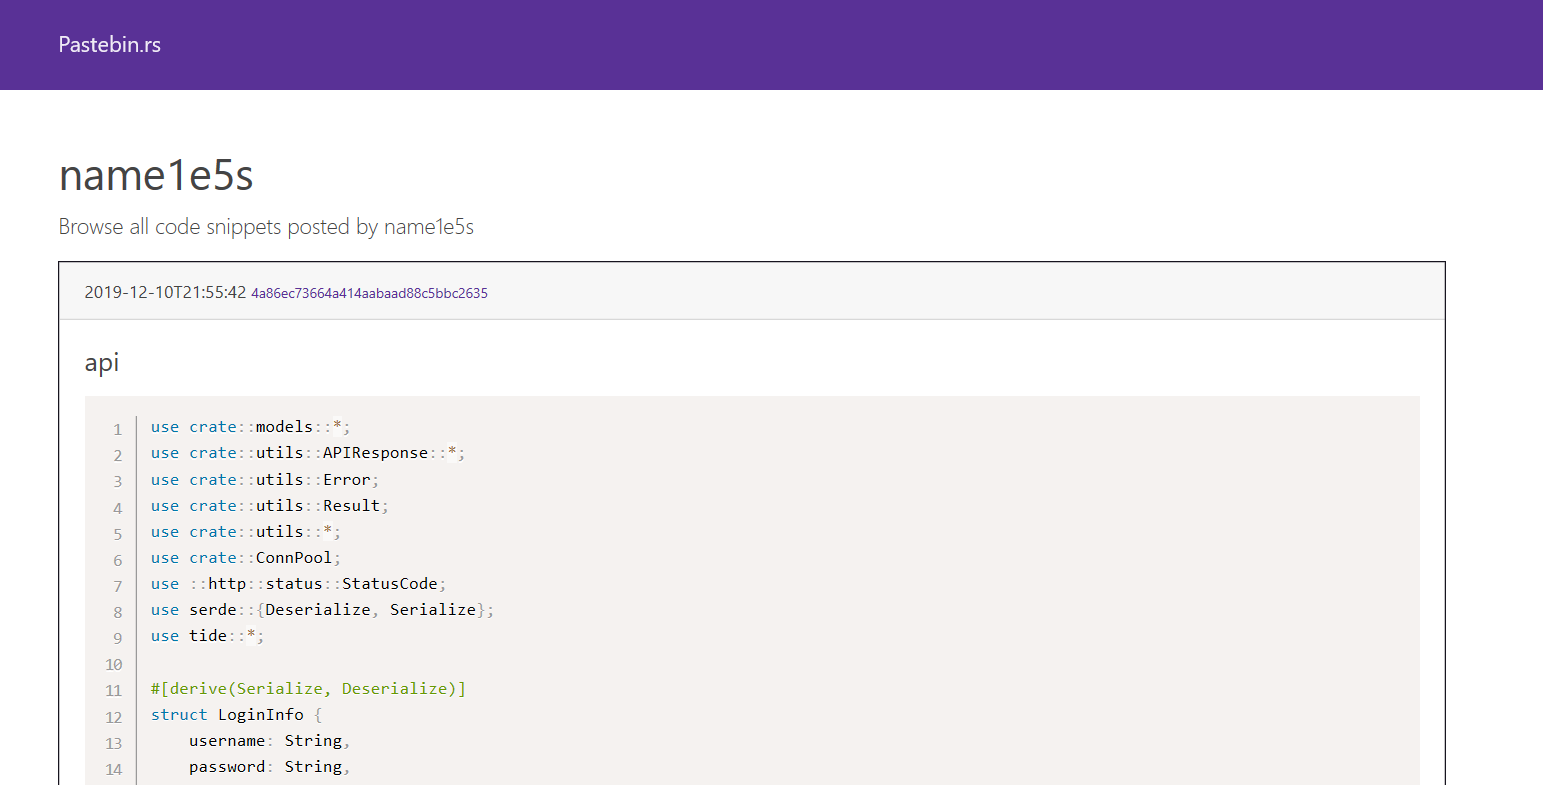
\includegraphics[width=.8\textwidth]{user}
    \caption{用户界面}
    \label{fig:user}
\end{figure}

在列表内点击任一 UUID,即可进入该代码片段对应的展示界面,如图~\ref{fig:paste}~。

\begin{figure}[!htbp]
    \centering
    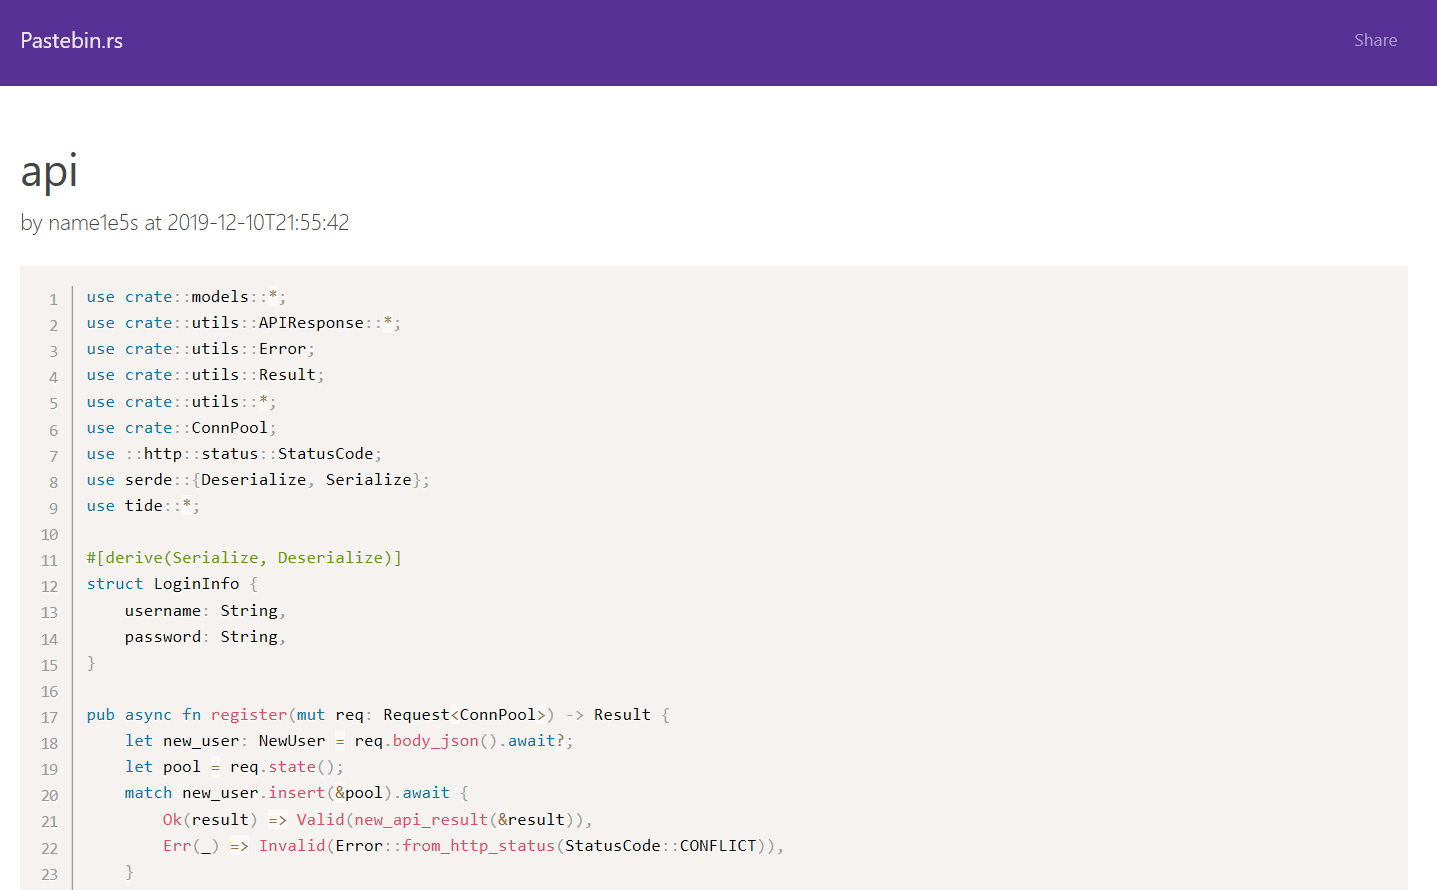
\includegraphics[width=.8\textwidth]{paste}
    \caption{代码片段界面}
    \label{fig:paste}
\end{figure}

点击右上角的 Share,弹出分享窗口,可以在这里复制连接或者获取二维码以供分享,如图~\ref{fig:share}~。

\begin{figure}[!htbp]
    \centering
    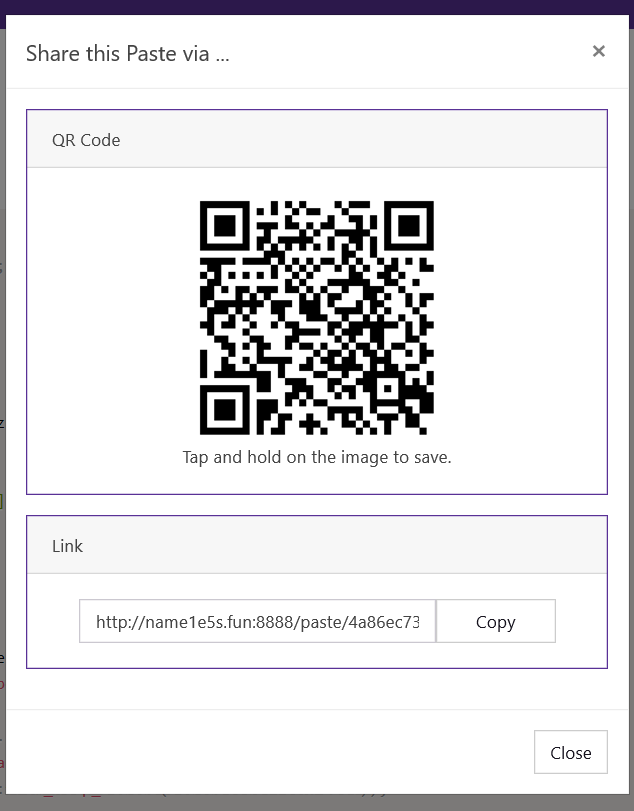
\includegraphics[width=.5\textwidth]{share}
    \caption{分享界面}
    \label{fig:share}
\end{figure}

\end{document}